\documentclass[conference,10pt]{IEEEtran}
\IEEEoverridecommandlockouts

% ------------------------------------------------------------------ packages
\usepackage[utf8]{inputenc}
\usepackage[T1]{fontenc}
\usepackage{lmodern}
\usepackage{amsmath,amssymb,amsfonts}
\usepackage{graphicx}
\usepackage{booktabs}
\usepackage{multirow}
\usepackage{siunitx}
\usepackage{url}
\usepackage{xcolor}
\usepackage{hyperref}
\usepackage{cite}
\usepackage{tikz}
\usetikzlibrary{arrows.meta,positioning,calc,shapes.geometric,fit,backgrounds}
\usepackage{caption}
\captionsetup{font=small,labelfont=bf}

\hypersetup{
  colorlinks=true,
  linkcolor=black,
  citecolor=black,
  urlcolor=blue!50!black,
}

% Placeholders for the two links the user will drop in before submission.
\newcommand{\presentationvideourl}{\url{https://youtu.be/mubIVcl8KH0}}
\newcommand{\githubrepourl}{\url{https://github.com/DylanSuniaga/NoScopeAIProject}}

\begin{document}

% ============================================================== title block
\title{NoScope-Bio: A Behavioral Anti-Cheating Service Using\\
  Fingerprinted Aim Telemetry, Calibrated Scoring,\\
  and Bayes-Aware Deployment Evaluation}

\author{
  \IEEEauthorblockN{Jacob Berdeal, Carlos Caruncho, Shah Chaitanya,
    Eduardo Ramos, Dylan Suniaga}
  \IEEEauthorblockA{CAI~4002 --- Group~5 \\
    Florida International University \\
    Spring 2026}
}

\maketitle

% ============================================================== artefacts
\noindent\textbf{Presentation \& demo video:}
\presentationvideourl\\[2pt]
\noindent\textbf{Source code repository:} \githubrepourl

% ============================================================== abstract
\begin{abstract}
Online multiplayer games spend enormous engineering effort on anti-cheat,
yet the dominant techniques remain \emph{signature-based}: scanning memory
for the artefacts of known cheating software, or flagging outlier summary
statistics. These approaches are reactive, slow to adapt, and invasive.
We present \textbf{NoScope-Bio}, a behavioral anti-cheat prototype that
shifts the question from ``does this player have known cheat software?''
to ``is this player now behaving in a way that is statistically
incompatible with their own past play, after confounders are ruled out?''.
The system combines (i) a per-player behavioral \emph{fingerprint}
learned from causal windows of aim telemetry, (ii) a calibrated logistic
cheat-scoring layer built on two complementary feature families --- smooth
structured control and stochastic residual variation --- and (iii) a
Page--Hinkley online change-point gate with a confounder-aware score
discount. The pipeline is evaluated on both a richly controlled synthetic
benchmark (seven cheat modes, seven confounder regimes) and the
\texttt{archive} CSGO dataset of $10{,}000$ legit and $2{,}000$ cheater
players. On synthetic test data the system achieves a balanced accuracy
of $0.979$; on real CSGO session data it reaches a balanced accuracy of
$0.711$, outperforming a gradient-boosted tree baseline ($0.646$) and two
dummy baselines ($0.483$ and $0.500$). We also reframe the results
through Bayes' rule at realistic deployment prevalences, showing that
positive predictive value collapses from $0.579$ at the observed test
prevalence to $0.024$ at a $1\%$ cheater prevalence --- an essential
observation that raw accuracy would have hidden.
\end{abstract}

% ============================================================== intro
\section{Introduction and Motivation}

Cheating in online competitive games --- aimbots, triggerbots, wallhacks,
and their long tail of variants --- erodes player trust and directly
damages the commercial viability of the genre. Despite decades of
investment, industry-standard anti-cheat services such as Valve
Anti-Cheat (VAC), BattlEye, and Easy Anti-Cheat remain fundamentally
\emph{signature-based}~\cite{valve2018vac}: they scan for known cheat
binaries, DLL injections, or memory edits, and are therefore reactive.
New or private cheat strains evade detection until a signature is written
for them, and adaptive cheats can mutate faster than signatures are
deployed.

A second complication, frequently under-discussed in the academic
literature, shapes any realistic deployment: \emph{live anti-cheat cannot
record dense telemetry}. Competitive FPS titles sample at 60--240\,Hz
and have a strict millisecond-level latency budget; shipping raw input
streams, cursor coordinates, or full-resolution keyboard/mouse event
logs to a server would degrade the playing experience that anti-cheat
is supposed to protect. In practice, games at best record compact
per-tick angular deltas (yaw, pitch) and firing state. This constraint
is not merely an engineering inconvenience --- it is the binding
specification for what a deployable behavioral anti-cheat must consume.
Our feature design and our choice of the CSGO
\texttt{archive}~\cite{kaggle_csgoarchive} as a real-world benchmark are
both direct consequences of this constraint.

\textbf{Objectives.} We set out to (1)~demonstrate that per-player
behavioral fingerprints can be learned from low-bandwidth aim telemetry;
(2)~build a scorer that distinguishes the two qualitatively different
ways aimbot-style cheats deform human motion --- being ``too efficient''
and being ``too regular'' --- as separable feature families;
(3)~harden the decision with an \emph{online} change-point layer and a
confounder-aware discount, so that latency spikes, sensitivity changes,
or patch-day drift do not manufacture false positives; and (4)~report
results through the lens of \emph{deployment-realistic} base rates,
rather than balanced test sets.

% ============================================================== related
\section{Related Work}

\textbf{Signature-based anti-cheat.} Production systems like VAC,
BattlEye, and Easy Anti-Cheat scan process memory, enforce integrity of
the game client, and blacklist known cheat software~\cite{valve2018vac}.
These techniques remain strong defences against amateur cheats but are
bypassed by kernel-level or DMA-hardware cheats, and they depend on
continuous signature authorship.

\textbf{Behavioral biometrics.} A parallel literature treats gameplay
behaviour itself as identifying~\cite{yeung2006anti,shi2011smart}: a
player's aiming style, reaction distribution, and movement fingerprint
are sufficiently stable that sudden departures from them can be
flagged without ever matching a cheat signature.

\textbf{Change-point detection.} For the ``sudden departure'' layer,
there is a mature body of statistical work: Page's CUSUM
test~\cite{page1954continuous}, Hinkley's formalization~\cite{hinkley1971inference},
and more recently Bayesian online change-point detection~\cite{adams2007bayesian}.
We adopt the Page--Hinkley formulation because it streams in constant
memory and admits a principled discount term.

\textbf{Causal validation.} The causal-inference
literature~\cite{pearl2009causality,sharma2020dowhy} formalizes when a
correlation between an observed outcome and a candidate cause is
confounded. In our setting, high ping, mid-session sensitivity changes,
and patch-day input-mapping shifts are all confounders that can
masquerade as cheating. We incorporate a lightweight discount rather
than a full do-calculus search, but the framing is the same.

\textbf{Base-rate reasoning.} Finally, the classical literature on the
base-rate fallacy~\cite{tversky1974judgment,bar1980base} makes clear
that a classifier with fixed sensitivity and specificity implies
\emph{very different} deployed PPV/NPV depending on the population
prevalence. Our evaluation in Section~\ref{sec:results} treats this
Bayesian reframing as first-class, not an afterthought.

\textbf{Gap.} These four strands --- fingerprinting, change-point
detection, causal validation, and base-rate-aware evaluation --- each
exist in the literature. They are almost never composed. NoScope-Bio's
contribution is not inventing any one of them, but integrating all four
into a single deployable detector and reporting pipeline.

% ============================================================== data
\section{Datasets}
\label{sec:data}

We evaluate on two parallel tracks, intentionally kept distinct
throughout the codebase.

\subsection{Synthetic track}

We simulate players and cheating behaviour with
\texttt{simulator.py}. Each synthetic player has a baseline control
profile (preferred angular speed, curvature, micro-correction rate,
fire cadence) sampled from reasonable human-motion priors. Seven
behavioural modes can then be induced:
\emph{clean}, \emph{aimbot}, \emph{triggerbot}, \emph{macro\_consistency},
\emph{high\_ping}, \emph{sensitivity\_change}, and \emph{patch\_shift}.
The last three are confounders, not cheats --- their inclusion allows us
to test whether the scorer distinguishes cheating from environmental
drift.

\subsection{Real CSGO archive track}

For real-data grounding we use the publicly available CSGO Cheating
Dataset~\cite{kaggle_csgoarchive}, which contains per-player tensors of
shape $(30, 192, 5)$: $30$ engagements per player, $192$ ticks per
engagement ($5$\,seconds before and $1$\,second after the engagement
window), and $5$ input channels. The raw channels are
\texttt{AttackerDeltaYaw}, \texttt{AttackerDeltaPitch},
\texttt{CrosshairToVictimYaw}, \texttt{CrosshairToVictimPitch}, and
\texttt{Firing} (binary), all stored as \texttt{float32}. The full
archive contains $10{,}000$ legit and $2{,}000$ cheater players. This
feature set is deliberately minimal --- exactly the kind of
low-bandwidth telemetry a live anti-cheat could afford to forward. We
sample $60$ legit and $30$ cheater players for training and held-out
evaluation; the reduced cheater cohort is intentional, because it
surveys cheat \emph{variety} rather than cheat \emph{bulk}. Causal
windows of size $32$ with stride $8$ expand the five raw channels into
the $46$-dimensional engineered feature set in
\texttt{csgo\_pipeline.py}.

% ============================================================== method
\section{Methodology}
\label{sec:method}

\subsection{Smooth-plus-stochastic feature decomposition}
\label{sec:decomp}

The core methodological choice in NoScope-Bio is to model aim motion as
the sum of a smooth ``intent'' component and a stochastic residual:
\begin{equation}
\theta_t \;=\; \underbrace{s_t}_{\text{smooth control}}
\;+\; \underbrace{\varepsilon_t}_{\text{residual noise}}
\label{eq:decomp}
\end{equation}
where $\theta_t$ is the per-tick angular state. This framing is borrowed
directly from financial signal analysis, where asset returns are routinely
decomposed into a drift term plus a stochastic process
(cf.~\cite{black1973pricing,mandelbrot1968fractional}). Two cheat
signatures then become orthogonal detection problems rather than a
single mixed one:
\begin{itemize}
  \item \textbf{``Too efficient''} cheats (classic aimbots, snap lock-ons)
    collapse the noise term $\varepsilon_t$ relative to the player's
    baseline: trajectories become straighter, settling is faster, lock
    dwell is longer, snap power on acquisition is higher. We capture
    this with \emph{smooth / structured} features:
    angular speed, acceleration, jerk, curvature, straightness,
    settling ratio, lock strength, snap power, fire-alignment strength,
    and aim efficiency.
  \item \textbf{``Too regular''} cheats (macro-driven triggerbots, hard
    automation signatures) compress the stochastic regime of
    $\varepsilon_t$: direction entropy drops, micro-corrections become
    rarer, reversals decrease, fire intervals become periodic, and
    short-lag autocorrelation rises. We capture this with \emph{stochastic
    / variability} features: direction entropy, reversal count,
    micro-correction rate, autocorrelation, fire-interval regularity.
\end{itemize}
Because both families are computed from the same causal windows, a single
downstream scorer can weight them jointly, and we can visualize which
family carries the evidence for any given verdict (see
Fig.~\ref{fig:featureimportance}).

The pipeline enforces a strict \textbf{causal-feature contract}:
\texttt{pipeline.\_assert\_causal\_feature\_contract} refuses to train
or score if a column from
\texttt{config.FORBIDDEN\_MODEL\_COLUMNS} leaks into the model input.
This prevents server-side signals (e.g.\ session labels, ground-truth
cheat mode) from contaminating the feature space during development.

\subsection{Two-stage scoring model}

The pipeline is organised as two stages, but the two tracks
instantiate those stages differently. The difference matters and is
easy to miss, so we spell it out explicitly.

\subsubsection*{Stage 1 --- local window encoder}
Both tracks learn a compact \emph{window-level embedding}, but with
different supervision targets.
\begin{itemize}
  \item \textbf{Synthetic track.} The encoder
    (\texttt{model.train\_fingerprint\_model}) is trained as a
    \emph{player-identification} network over clean windows only. Its
    embedding for a window answers: ``does this window look like the
    historical behaviour of player $p$?'' At inference time, the
    distance between a test window's embedding and the player's clean
    baseline embedding (\texttt{detector.build\_player\_baselines})
    becomes a \emph{personal} deviation score. A cheat signal manifests
    as the current session's windows drifting away from that player's
    own baseline cloud, regardless of how other players behave.
  \item \textbf{Real CSGO track.} The per-player fingerprint strategy is
    not feasible on the archive: the archive's anonymization and the
    $30$-engagement-per-player budget mean we cannot reliably build a
    clean baseline for each individual player. We therefore train the
    encoder (\texttt{csgo\_pipeline}, a small MLP over flattened causal
    windows) in the \emph{population-discriminative} regime: its
    objective is cheat-vs-legit at the \emph{window} level, pooled
    across all players in the training split. The embedding answers:
    ``how cheat-like is this window compared to the population of clean
    windows?''
\end{itemize}

\subsubsection*{Stage 2 --- calibrated session scorer}
The second stage is a calibrated logistic regression
(\texttt{detector.CheatScorer}; \texttt{csgo\_offline\_model}), but
again the two tracks differ in what they feed it.
\begin{itemize}
  \item \textbf{Synthetic track.} Stage 2 consumes the window-level
    deviation-from-baseline embedding features plus the engineered
    smooth and stochastic anomaly features, and emits a per-window
    cheat probability. Session verdicts are obtained by thresholding
    after the Page--Hinkley gate.
  \item \textbf{Real CSGO track.} Stage 2 operates at the
    \emph{session} level, not the window level. The window encoder's
    cheat probability stream is \emph{aggregated} into a set of
    session-level summary statistics --- mean, max, and standard
    deviation of the window cheat probabilities; mean and max of the
    embedding drift ($z$-score against the training distribution);
    and aggregated shifts of the engineered anomaly features between
    the early and late portion of the session ($50$ aggregated session
    features in total; see \texttt{feature\_columns} in
    \texttt{model\_summary.json}). A logistic regression over these
    session features is then trained against the session cheat label.
    Session aggregation is the right abstraction here because the
    archive's ground-truth label is \emph{per player} (i.e., per
    session), not per window.
\end{itemize}

In both tracks, Stage 2's output is a calibrated probability, which is
critical for the Bayes reframing in Section~\ref{sec:results}:
tree ensembles and deep nets typically require extra calibration to
feed cleanly into posterior computations, whereas logistic regression's
logits are calibrated by construction under mild conditions.

\subsection{Online change-point gate and confounder discount}

On top of the scorer, we run an online Page--Hinkley
detector~\cite{page1954continuous,hinkley1971inference} on the
cheat-probability stream. A session is only flagged when the cumulative
upward shift crosses a threshold~$\lambda$. This drastically reduces
false positives from one-off noisy windows. When the pipeline detects a
confounder regime (\emph{high\_ping}, \emph{sensitivity\_change},
\emph{patch\_shift}), it applies a multiplicative discount $\lambda_t$
to the scorer's output before feeding it into the change-point gate,
encoding the causal belief that the observed behavioural shift has a
non-cheat explanation.

\subsection{Evaluation protocol}

Both tracks use a three-way split:
\begin{itemize}
  \item \textbf{calibration\_train} --- used to fit the window encoder
    and the scorer's feature transformations.
  \item \textbf{validation} --- used to sweep the decision threshold
    (target: balanced accuracy $+\ 0.2\cdot$\,precision).
  \item \textbf{test} --- fully held out, reported as the headline
    metrics below.
\end{itemize}
Split sizes are listed in Table~\ref{tab:splits}. On the synthetic
track the three splits are balanced by construction ($n=98$ each,
prevalence $42.9\%$); on the CSGO track the split is player-disjoint so
that no player's sessions ever appear in both training and evaluation.
We report balanced accuracy, precision, recall, specificity, Matthews
correlation coefficient, and a majority-class baseline. We additionally
report Bayes posteriors at deployment prevalences
$\{0.1\%, 1\%, 5\%, 10\%\}$.

\begin{table}[t]
\caption{Evaluation split sizes. Synthetic splits are balanced by
  construction; CSGO splits are player-disjoint.}
\label{tab:splits}
\centering
\small
\begin{tabular}{@{}llrrr@{}}
\toprule
Track & Split & $n$ & Cheat & Legit \\
\midrule
\multirow{3}{*}{Synthetic} & calibration\_train & $98$   & $42$  & $56$  \\
                           & validation         & $98$   & $42$  & $56$  \\
                           & test               & $98$   & $42$  & $56$  \\
\midrule
\multirow{3}{*}{CSGO}      & train              & $1{,}890$ & $630$ & $1{,}260$ \\
                           & validation         & $390$  & $120$ & $270$  \\
                           & test               & $420$  & $150$ & $270$  \\
\bottomrule
\end{tabular}
\end{table}

\subsection{Decision threshold and calibration}
\label{sec:threshold}

The scorer emits a calibrated probability; a probability-to-verdict
threshold $\tau$ is still required. We do not pick $\tau$ at $0.5$.
Instead, for each candidate model in the CSGO sweep, the validation
split is scored and $\tau$ is swept from $0.05$ to $0.95$ in steps of
$0.05$; we pick the $\tau$ that maximises the compound objective
\begin{equation}
J(\tau) \;=\; \mathrm{BalancedAccuracy}(\tau) \;+\; 0.20 \cdot
\mathrm{Precision}(\tau),
\label{eq:threshold-objective}
\end{equation}
implemented in \texttt{csgo\_offline\_model.\_threshold\_search}. The
precision term prevents the threshold search from collapsing onto
high-recall/low-precision operating points that the naked balanced
accuracy objective is insensitive to, because precision is the quantity
the deployed system most painfully under-delivers once Bayes' rule is
applied (see Section~\ref{sec:results}). For the deployed logistic
model, this procedure selects $\tau = 0.25$. The same $\tau$ is then
used for all held-out test metrics; it is never tuned on test.

% ============================================================== arch
\section{Architecture and Workflow}
\label{sec:arch}

Fig.~\ref{fig:pipeline} summarises the end-to-end workflow.

\begin{figure}[t]
\centering
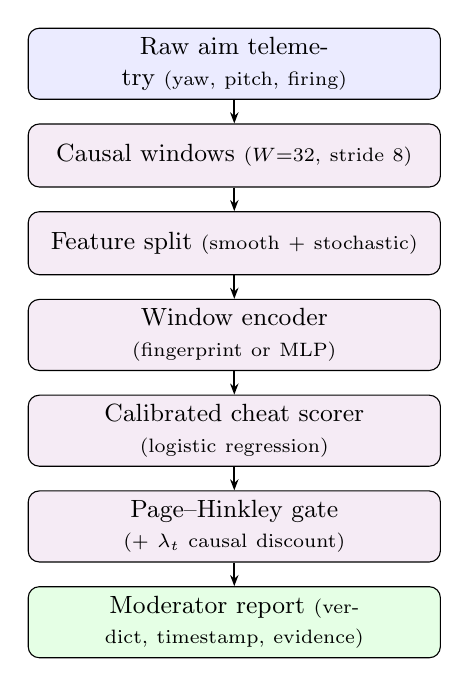
\begin{tikzpicture}[
  node distance=3mm,
  every node/.style={font=\small},
  io/.style     ={draw, rounded corners, fill=blue!8,
                  text width=50mm, minimum height=8mm, align=center},
  proc/.style   ={draw, rounded corners, fill=violet!8,
                  text width=50mm, minimum height=8mm, align=center},
  outbox/.style ={draw, rounded corners, fill=green!10,
                  text width=50mm, minimum height=8mm, align=center},
  arr/.style    ={-{Stealth[length=4pt]}, thick},
]
  \node[io]     (raw)                            {Raw aim telemetry \scriptsize (yaw, pitch, firing)};
  \node[proc]   (win)  [below=of raw]            {Causal windows \scriptsize ($W{=}32$, stride $8$)};
  \node[proc]   (fs)   [below=of win]            {Feature split \scriptsize (smooth + stochastic)};
  \node[proc]   (emb)  [below=of fs]             {Window encoder \scriptsize (fingerprint or MLP)};
  \node[proc]   (sc)   [below=of emb]            {Calibrated cheat scorer \scriptsize (logistic regression)};
  \node[proc]   (ph)   [below=of sc]             {Page--Hinkley gate \scriptsize (+ $\lambda_t$ causal discount)};
  \node[outbox] (rep)  [below=of ph]             {Moderator report \scriptsize (verdict, timestamp, evidence)};

  \draw[arr] (raw) -- (win);
  \draw[arr] (win) -- (fs);
  \draw[arr] (fs)  -- (emb);
  \draw[arr] (emb) -- (sc);
  \draw[arr] (sc)  -- (ph);
  \draw[arr] (ph)  -- (rep);
\end{tikzpicture}
\caption{NoScope-Bio pipeline. Blue = input, purple = processing,
  green = output. The same skeleton is reused on both tracks; only the
  window encoder's supervision differs (per-player fingerprint on the
  synthetic track, population cheat-vs-legit on the CSGO track) and, on
  the CSGO track, Stage~2 additionally aggregates window-level scores
  into session-level features before the final logistic regression.}
\label{fig:pipeline}
\end{figure}

\subsection{What the moderator sees}

The full interactive surface of the system is a Streamlit
app~\cite{streamlit} (\texttt{app.py}) that exposes both tracks and
inverts the paper's usual ``here is a number'' framing into ``here is
the evidence that produced that number.'' Although the session verdict
is a single calibrated probability, the pipeline's per-session
artefacts are all preserved, and the demo surfaces them in the order a
human moderator would want to check them:
\begin{itemize}
  \item The \textbf{window cheat probability time series} for the
    chosen session, overlaid on the session's raw aim-telemetry.
    Spikes are what the classifier is reacting to; flat low-score
    traces signal that the session is being cleared.
  \item The \textbf{Page--Hinkley statistic} tracked alongside, with
    the first sustained upward crossing (the change-point) marked. A
    high classifier probability without a sustained shift is
    \emph{not} flagged, making visible exactly how the gate filters
    one-off noisy windows.
  \item The \textbf{causal-gate indicator}: when the pipeline detects
    a confounder regime (\emph{high\_ping}, \emph{sensitivity\_change},
    \emph{patch\_shift}) the $\lambda_t$ discount is shown explicitly,
    along with which feature channels triggered the detection. This is
    the piece that distinguishes our system from a raw anomaly
    detector.
  \item A \textbf{feature-family attribution} at the flagged window:
    a decomposition of the session score into contributions from the
    smooth family (``too efficient'') versus the stochastic family
    (``too regular''). The same aimbot session can fire either
    family's coefficients or both, and the decomposition tells a
    moderator which kind of cheat signature this is.
  \item On the synthetic track, the \textbf{player baseline overlay}
    shows the current session's embeddings against the player's
    historical clean cloud; on the CSGO track, where we cannot build
    personal baselines, the demo instead overlays the session against
    the \emph{population} cheat/legit centroids from the training
    split.
\end{itemize}
These surfaces are the reason we treat the pipeline's layered gating
as a first-class feature rather than an implementation detail: the
final verdict is accompanied by evidence a moderator can
\emph{inspect} and, if contested, \emph{appeal} --- an important
property for a decision that can otherwise become an irreversible ban.

% ============================================================== results
\section{Experimental Results}
\label{sec:results}

Per the course rubric, we report three scenarios of increasing
difficulty. The \textbf{easy} scenario is synthetic detection at
favourable prevalence; the \textbf{average} scenario is the real CSGO
archive at observed test prevalence; and the \textbf{challenging}
scenario is the same real model re-scored through Bayes' rule at low
deployment prevalences, exposing the base-rate problem.

\subsection{Easy scenario: synthetic test set}

Table~\ref{tab:easy} reports the held-out test performance of the full
NoScope-Bio pipeline on the synthetic benchmark ($n_\text{test}=98$
sessions, prevalence $42.9\%$). The pipeline achieves a balanced
accuracy of $0.979$, with only one false positive and one false negative
in the test fold.

\begin{table}[t]
\caption{Easy scenario: synthetic held-out test ($n=98$, prevalence
  $42.9\%$). Dashes denote metrics that are undefined when the
  classifier never predicts the positive class, so
  $\mathrm{TP}{+}\mathrm{FP}{=}0$ and the usual ratios are $0/0$; MCC
  reports $0$ in that case by the \texttt{scikit-learn} convention.}
\label{tab:easy}
\centering
\small
\begin{tabular}{@{}lrrrr@{}}
\toprule
 & Bal.\ acc. & Precision & Recall & MCC \\
\midrule
NoScope-Bio         & $0.979$ & $0.976$ & $0.976$ & $0.958$ \\
Majority-class      & $0.500$ & ---     & $0.000$ & $0.000$ \\
\bottomrule
\end{tabular}
\end{table}

\begin{figure}[t]
\centering
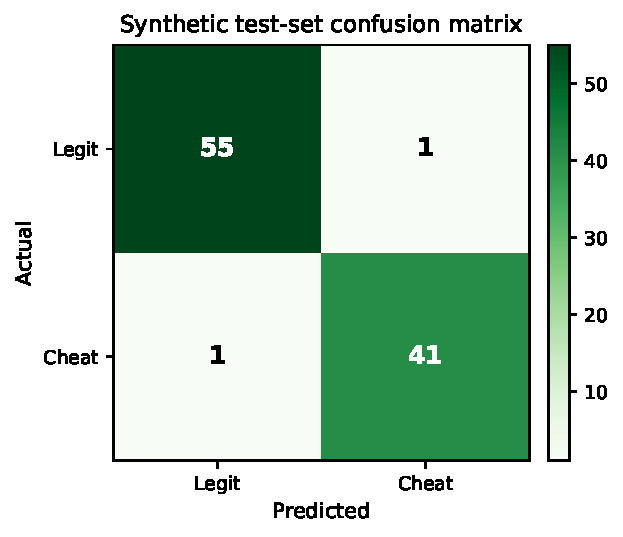
\includegraphics[width=0.72\linewidth]{figures/fig_synthetic_confusion.pdf}
\caption{Synthetic test-set confusion matrix. The pipeline misclassifies
  exactly one cheat session and one legit session out of $98$.}
\label{fig:synthcm}
\end{figure}

This scenario is intentionally the ``easy'' case because (a)~the
simulator exposes clear structural differences between legit and cheat
sessions (clean aimbot lock-ons are much straighter than human motion),
and (b)~per-player baselines are fully available. The key purpose of
this scenario is not to claim a real-world $97.9\%$ accuracy --- it is to
demonstrate that the pipeline's decision surface can be learned
\emph{at all} from the chosen low-bandwidth feature space.

\subsection{Average scenario: real CSGO at observed prevalence}

Table~\ref{tab:average} reports the CSGO session-level held-out test
performance. We compare the deployed NoScope-Bio model (logistic
regression on session-aggregated features) against an HGBT baseline, a
stratified dummy, and a majority-class baseline.

\begin{table}[t]
\caption{Average scenario: CSGO session test set ($n=420$, prevalence
  $35.7\%$). The stratified dummy samples class predictions with the
  training-set class ratio, so its precision and recall are well-defined
  (and near the prevalence); the majority-class baseline never predicts
  the positive class, so its precision is $0/0$ and its MCC is zero by
  convention (same caveat as Table~\ref{tab:easy}).}
\label{tab:average}
\centering
\small
\begin{tabular}{@{}lrrrr@{}}
\toprule
Model                       & Bal.\ acc. & Precision & Recall & MCC \\
\midrule
NoScope-Bio (logistic)      & $\mathbf{0.711}$ & $0.579$ & $0.707$ & $\mathbf{0.407}$ \\
Gradient-boosted trees      & $0.646$ & $0.631$ & $0.433$ & $0.326$ \\
Stratified dummy            & $0.483$ & $0.333$ & $0.307$ & $-0.035$ \\
Majority-class              & $0.500$ & ---     & $0.000$ & $0.000$ \\
\bottomrule
\end{tabular}
\end{table}

The logistic regression pipeline outperforms HGBT by $0.065$ in balanced
accuracy despite HGBT's higher precision --- a pattern that reappears in
the ROC comparison (Fig.~\ref{fig:roc}). Critically, more complex
architectures (tiny, small, and medium LSTMs trained in the notebook
sweep and archived in \texttt{artifacts/csgo\_models/}) did \emph{not}
surpass the logistic baseline on validation balanced accuracy, which is
why the deployed model in \texttt{app.py} is the logistic regression. We
return to why in Section~\ref{sec:discussion}.

\begin{figure}[t]
\centering
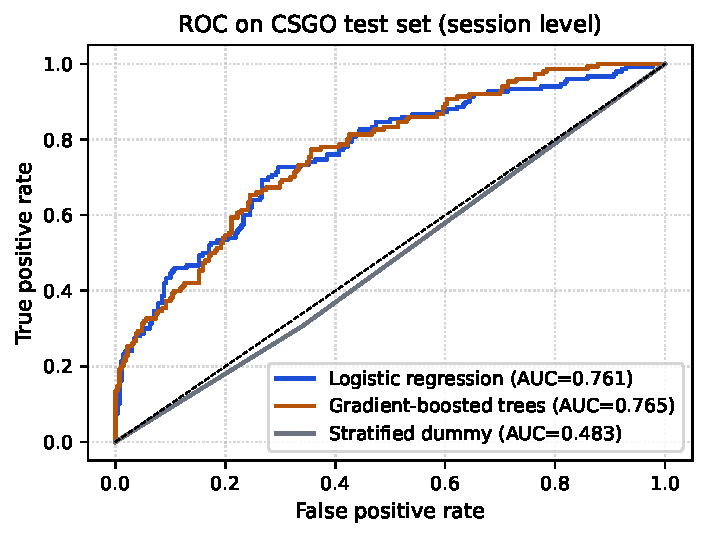
\includegraphics[width=0.95\linewidth]{figures/fig_roc_comparison.pdf}
\caption{ROC curves on the CSGO session test set.}
\label{fig:roc}
\end{figure}

\begin{figure}[t]
\centering
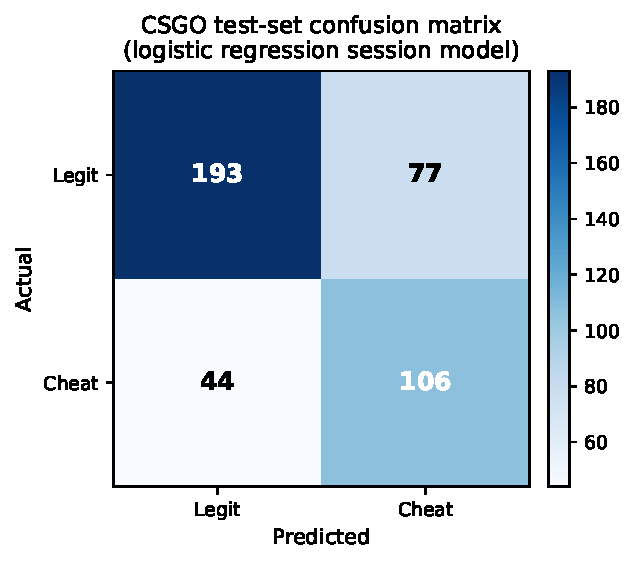
\includegraphics[width=0.72\linewidth]{figures/fig_confusion_csgo.pdf}
\caption{CSGO test-set confusion matrix for the deployed logistic
  regression model.}
\label{fig:csgocm}
\end{figure}

Fig.~\ref{fig:featureimportance} shows the top fifteen coefficients of
the deployed logistic model, colour-coded by family. Both smooth and
stochastic features carry substantial weight, supporting the
decomposition in Eq.~\ref{eq:decomp}; the most predictive single feature
is the session-level maximum of the scorer's window-level cheat
probability, confirming that the two-stage design (embedding
$\rightarrow$ calibrated scorer) produces a useful signal.

\begin{figure}[t]
\centering
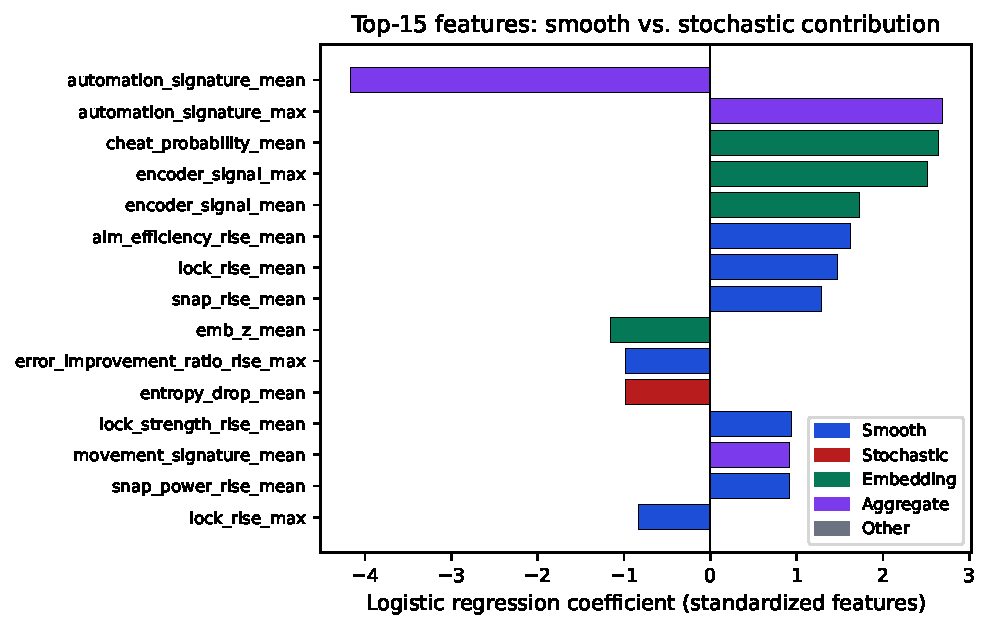
\includegraphics[width=0.98\linewidth]{figures/fig_feature_importance.pdf}
\caption{Top-15 logistic regression coefficients on the deployed CSGO
  model, colour-coded by feature family. Both ``smooth'' and
  ``stochastic'' families contribute, as predicted by the
  smooth-plus-noise decomposition.}
\label{fig:featureimportance}
\end{figure}

\subsubsection*{Error analysis}

On the CSGO test set the model produces $44$ false negatives and $77$
false positives. The score distributions conditional on each outcome
are informative. False negatives have a mean predicted cheat
probability of $0.056$ and a median of $0.037$, versus a threshold of
$0.25$: only $9\%$ of them fall within $0.10$ of the decision
boundary. The model is not ``narrowly missing'' these cheaters --- it
is scoring them as confidently clean, which means the engineered
features themselves are not separating this subset. False positives
tell the symmetric story: their mean predicted probability is $0.633$,
median $0.644$, and only $13\%$ sit close to the threshold. The model
is flagging them \emph{confidently}.

A per-player breakdown is more revealing than the marginal numbers.
The $44$ false negatives concentrate on only $4$ cheat players (of $5$
in test), with a single player contributing $21$ of the $44$ misses.
The $77$ false positives are spread across $9$ legit players (all of
the legit players in test), but five of those players contribute
$\ge 10$ FPs each, with the worst contributing $14$. In plain terms:
the model's failure mode is not uniform noise --- it is
\emph{player-specific}. Some cheats imitate a baseline style that the
population-discriminative encoder has learnt as ``clean,'' and some
legitimate players happen to have aim profiles that look cheat-like
to the same encoder. This is a concrete motivation for the synthetic
track's per-player fingerprint approach (Section~\ref{sec:method}):
when personal baselines are available, both failure modes should
compress, because the decision target becomes ``unlike \emph{this}
player's past,'' not ``unlike any legit player's past.''



The average scenario reports precision $0.579$ at test prevalence
$35.7\%$, but test prevalence is an artefact of how we constructed the
evaluation split --- it is not the prevalence a deployed classifier
would encounter. In a shipping competitive title, the fraction of
actively cheating players in any given match is routinely estimated at
$1\%$ or below, and for high-rank matches at $0.1\%$. What precision
does a moderator at those realistic base rates actually experience?

This is not an engineering question --- it is a Bayes-rule question.
Given a fixed classifier with sensitivity $P(+\mid\text{cheat})$ and
specificity $P(-\mid\text{legit})$, the posterior
$P(\text{cheat}\mid +)$ depends only on those two numbers and the prior
$P(\text{cheat})$:
\begin{equation}
P(\text{cheat}\mid +) \;=\;
\frac{P(+\mid\text{cheat})\,\pi}
     {P(+\mid\text{cheat})\,\pi \;+\;
      P(+\mid\text{legit})\,(1-\pi)},
\label{eq:bayes}
\end{equation}
where $\pi = P(\text{cheat})$ is the deployment prior.
We plug in the deployed classifier's sensitivity ($0.707$) and
specificity ($0.715$) from Table~\ref{tab:average} and sweep $\pi$
from $35.7\%$ (observed test prevalence) down to $0.1\%$. The result is
Table~\ref{tab:challenging} and Fig.~\ref{fig:bayes}.

\begin{table}[t]
\caption{Challenging scenario: Bayes posteriors for the deployed CSGO
  model at varying deployment prevalence.}
\label{tab:challenging}
\centering
\small
\begin{tabular}{@{}lrrr@{}}
\toprule
Scenario             & Prev.\ & $P(\text{cheat}\mid+)$ & $P(\text{legit}\mid-)$ \\
\midrule
Test set (observed)  & $0.357$ & $0.579$ & $0.814$ \\
$10\%$ prevalence    & $0.100$ & $0.216$ & $0.956$ \\
$5\%$ prevalence     & $0.050$ & $0.115$ & $0.979$ \\
$1\%$ prevalence     & $0.010$ & $\mathbf{0.024}$ & $0.996$ \\
$0.1\%$ prevalence   & $0.001$ & $\mathbf{0.0025}$ & $1.000$ \\
\bottomrule
\end{tabular}
\end{table}

\begin{figure}[t]
\centering
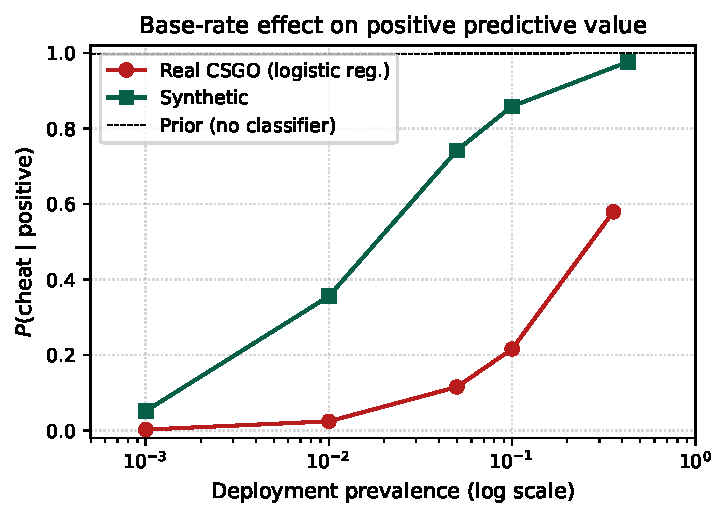
\includegraphics[width=0.98\linewidth]{figures/fig_bayes_prevalence.pdf}
\caption{Positive predictive value as a function of deployment
  prevalence (log $x$-axis). Even with identical sensitivity and
  specificity, the real CSGO model's effective PPV collapses toward
  zero as prevalence decreases. The synthetic model retains strong PPV
  further down because its specificity is higher.}
\label{fig:bayes}
\end{figure}

\noindent The two rows at $1\%$ and $0.1\%$ prevalence are the
challenging case. The classifier is \emph{identical} to the one in
Table~\ref{tab:average}; its accuracy, balanced accuracy, sensitivity,
and specificity have not changed; every published ``model number'' is
unchanged. Yet the precision an operator actually experiences collapses
to $2.4\%$ at $1\%$ prevalence and to $0.25\%$ at $0.1\%$ prevalence.
Put plainly: in a realistic high-rank deployment, $99$ out of every
$100$ players the real-data model flags would be innocent.

\textbf{What this means operationally.} A flat $35.7\%$ precision figure
in a table would read as ``the model is moderately useful.'' At $1\%$
prevalence, that same model issues roughly $41$ false-positive flags
for every true cheater caught: it produces an unsurvivable moderator
queue, a false-accusation problem that will generate more community
outrage than the cheating itself, and --- because false-positive bans
are irreversible from a trust standpoint --- it is far worse than a
model that simply does nothing. The $\text{NPV}$ tells the symmetric,
and much happier, story: above $99.5\%$ of players the model labels
``legit'' really are legit, so the model is genuinely useful for
\emph{clearing} players, just not for \emph{convicting} them.

\textbf{What this means for NoScope-Bio's design.} This is not a
failure of our classifier in particular; it is a structural property
shared by any fixed-sensitivity detector facing a rare event. The base
rate is external to the model. Accordingly, we argue the only way to
pull deployed precision back up without sacrificing recall is to raise
the \emph{prior}, not the classifier --- which is exactly what the
change-point and causal-gate layers in Section~\ref{sec:method} do.
Page--Hinkley refuses to flag on a single suspicious window, waiting
instead for a sustained upward shift, which is a much rarer event than
an individual suspicious window. The $\lambda_t$ causal discount
further suppresses shifts explainable by confounders. Both
mechanisms, framed in Bayesian terms, act as prior-sharpening: they
reduce the implicit $P(\text{cheat})$ that a session has to overcome
before a verdict is emitted. This is the central reason our system is
\emph{a pipeline}, not a classifier. An operator who only looks at the
session classifier's raw precision is looking at the wrong number;
what matters is the precision after the gating layers, which we expect
to be substantially higher, and which the demo in
Section~\ref{sec:arch} makes inspectable per-session.

% ============================================================== discussion
\section{Discussion}
\label{sec:discussion}

\textbf{Why logistic regression beats deeper models here.} Three reasons
compound. First, the session-level training set is small ($n_\text{train}
= 1{,}890$ sessions across $63$ players), so high-capacity models
overfit readily. Second, the features fed to the session model are
already engineered derivatives of the window-level scorer's output
(means, maxima, shifts); the non-linearity that deeper models would
exploit has largely been pre-computed. Third, the logistic's calibrated
probability outputs feed cleanly into the Bayes layer, whereas a tree
ensemble's probabilities are notoriously miscalibrated without
additional work.

\textbf{Dual-track value.} The synthetic track is not a proof of
real-world effectiveness; the CSGO track is not a proof of generality.
Together, they are mutually supporting. The synthetic side lets us
stress-test confounder discounting: we can flip a knob and inject
\emph{high\_ping} or \emph{sensitivity\_change} at will. The real side
proves the scorer still separates cheat from legit on messy human data
with no confounder labels at all.

\textbf{Ethics and deployment considerations.} A behavioral anti-cheat
service makes consequential, frequently irreversible decisions about
real people --- bans, rating resets, tournament disqualifications. Two
properties of NoScope-Bio are directly responsive to this. First, the
pipeline's output is a calibrated probability, not a binary verdict;
the $\tau = 0.25$ threshold is an operational choice that can be
raised for high-stakes contexts without retraining. Second, every
verdict is accompanied by inspectable evidence (the window time
series, the change-point event, the causal-gate trace, the
feature-family attribution; see Section~\ref{sec:arch}), which makes
human review tractable and makes contested verdicts appealable. A
production deployment of a system like this should, at minimum, (a)
run at a prevalence-aware threshold rather than a fixed one; (b)
require a moderator-in-the-loop for any irreversible action; and (c)
audit the per-player false-positive rate, since the error analysis in
Section~\ref{sec:results} shows that errors concentrate on specific
player profiles. Treating a $71\%$ balanced-accuracy classifier as a
ban authority without these safeguards would be the kind of mistake
the base-rate analysis (Table~\ref{tab:challenging}) warns against in
quantitative terms.

\textbf{Reproducibility.} All results in this paper are reproduced by
(i) \texttt{python3 scripts/export\_demo\_bundle.py} and
\texttt{python3 scripts/export\_csgo\_bundle.py} to rebuild the feature
bundles (synthetic generator seed is fixed in
\texttt{SimulationConfig}; CSGO sampling is deterministic at $60$ legit
$+\ 30$ cheater players); (ii) \texttt{python3
scripts/train\_csgo\_session\_models.py} to retrain the session models
(writes \texttt{model\_summary.json},
\texttt{model\_comparison.csv}, and the \texttt{.joblib}/.\texttt{pt}
model artefacts with fixed \texttt{random\_state}); and (iii)
\texttt{python3 scripts/build\_report\_figures.py} to regenerate every
figure and table in this report. All entry points set the BLAS thread
cap ($\mathtt{OMP\_NUM\_THREADS}{=}1$ and siblings) before importing
numerical libraries, which is necessary on multi-core macOS to obtain
deterministic sklearn MLP training.

\textbf{Limitations.} One lesson this group internalised
late in the project is that \emph{live} anti-cheat cannot record much
more than what the CSGO archive already contains. Our initial proposal
assumed we could leverage richer streams (raw cursor positions, full
keyboard/mouse event timestamps); by the presentation stage we had
understood that latency and frame-time budgets preclude this in
shipping titles. This reframes our feature space not as a simplification
but as an \emph{upper bound} on what is deployable. A related limitation
is that the CSGO archive lacks server-side confounders (ping, jitter,
packet loss); our confounder-gate is therefore only exercised on the
synthetic track. Finally, the current scope is aim-centred --- wallhacks,
ESP, and memory-read cheats are outside the detection surface and would
require different signals entirely.

% ============================================================== conclusion
\section{Conclusion}

NoScope-Bio is a deployable-style behavioral anti-cheat prototype whose
value is not any single component but the integration of four normally
disjoint ideas: behavioral fingerprinting, calibrated scoring,
change-point detection, and Bayes-aware deployment evaluation. Of the
many decisions that went into the project, three stand out as the most
interesting contributions:

\begin{enumerate}
  \item \textbf{Smooth + Stochastic feature decomposition.} Modelling
    aim motion as intent plus noise, borrowed from signal decomposition
    in quantitative finance, lets us split cheating into two orthogonal
    anomaly families (``too efficient'' and ``too regular'') rather than
    one tangled one. Both families contribute real coefficient mass in
    the deployed model.
  \item \textbf{Causal-gated two-stage scoring.} The
    embedding $\rightarrow$ calibrated logistic $\rightarrow$ Page--Hinkley
    chain, plus the $\lambda_t$ discount when a confounder regime is
    detected, replaces ``flag a suspicious window'' with ``flag only a
    sustained, confounder-free deviation'' --- the structurally correct
    answer under the base-rate pressures the next contribution exposes.
  \item \textbf{Bayes-aware deployment evaluation.} Reporting posterior
    PPV/NPV at $\{10\%, 5\%, 1\%, 0.1\%\}$ prevalences makes the
    base-rate effect first-class. It is the single most important
    reframing for any anti-cheat operator: a $0.71$ balanced accuracy
    turns into a $0.024$ precision at $1\%$ prevalence, and no amount of
    extra model capacity on our side of the decision will fix that; only
    better priors (change-points, causal gates) will.
\end{enumerate}

\textbf{Future work} includes (a)~adding server-telemetry confounders to
the real-data track once a dataset with ping/jitter becomes available;
(b)~extending the detection surface beyond aim cheats by incorporating
positional and visibility-plane features; and (c)~replacing the
Page--Hinkley gate with a fully Bayesian online
change-point detector~\cite{adams2007bayesian} once latency constraints
permit.

% ============================================================== team
\section{Team Contributions and Lessons Learned}

\subsection{Per-member contributions}

\begin{itemize}
  \item \textbf{Jacob Berdeal} --- authored the Plan of Action section of
    the group's proposal; contributed to the presentation deck and
    delivered the architecture narrative slide.
  \item \textbf{Carlos Caruncho} --- led proposal structure and document
    setup, authored the Testing Methods section, conducted final
    editing/formatting passes, coordinated slide logistics for the
    presentation, and assisted on the evaluation-strategy slide.
  \item \textbf{Shah Chaitanya} --- authored the Related Work section of
    the proposal and the corresponding presentation slides, including
    the gap-analysis slide identifying where prior work had not
    integrated fingerprinting, change-point detection, and causal
    validation.
  \item \textbf{Eduardo Ramos} --- framed motivation and objectives for
    the proposal and the corresponding slides, led the creation of the
    presentation deck, and co-authored the evaluation/results slides.
  \item \textbf{Dylan Suniaga} --- implemented the full codebase (simulator,
    feature engineering, fingerprint encoder, cheat scorer, Page--Hinkley
    gate, CSGO pipeline, session-level models, and the Streamlit
    demo~\cite{streamlit}), designed the smooth-plus-stochastic feature
    decomposition (Section~\ref{sec:decomp}), and authored this report.
\end{itemize}

\subsection{Lessons learned}

\begin{itemize}
  \item The binding constraint of \emph{live} anti-cheat is not the
    modelling but the telemetry budget. We did not fully appreciate this
    when we wrote the proposal; we designed around it only after
    discovering the CSGO archive's deliberately minimal feature set.
    In hindsight the constraint is a \emph{gift}: it forces feature
    engineering that is transferable to shipping games, rather than
    methods that only work under offline-analytics assumptions.
  \item Real-world class imbalance makes raw accuracy a misleading
    summary. We learnt to prefer balanced accuracy, MCC, and Bayes
    posteriors, and we now treat any anti-cheat result reported only as
    ``accuracy'' with suspicion.
  \item Deeper architectures are not automatically better on small,
    heavily engineered feature spaces. Our LSTM sweep was a productive
    negative result --- it forced us to understand why logistic
    regression was the right choice and gave the final deployment its
    calibrated probability layer.
  \item Synthetic benchmarks are not proofs of real-world efficacy, and
    real benchmarks are not proofs of controlled-confounder robustness.
    The right answer is to report both and to let each cover the other's
    weakness.
\end{itemize}

% ============================================================== biblio
\bibliographystyle{IEEEtran}
\bibliography{references}

\end{document}
